\section{Introduction}
Networks of small interlocking pods appear as a common thread throughout
successful large-scale collaborations.
However, it remains unclear whether that network structure plays a causal role
in the success of those collaborations,
and whether the specific structural properties of that interlocking network matter.
Observational study suggests a correlation between properties such as degree,
structural efficiency, and structural inequality and the performance/productivity
of collaborations \cite{platt_network_2018}.
Numerical simulation suggests a causal relationship in a simplified theoretical
setting.
This chapter proposes an online experiment to bridge these two findings.


\section{Study Software}

In order to conduct studies of network deliberation online, I have modified the
free and open-source Loomio platform \cite{jackson_open_2016}
to implement network deliberation.
Loomio is a widely-used online deliberation platform which provides both
forum functionality (Figure \ref{fig:reply})
and various forms of voting, including ranked-choice (Figure \ref{fig:vote}).
Loomio is popular among grassroots organizations and worker-owned cooperatives
(Loomio itself is a worker-owned cooperative).
Loomio was chosen for its combination of built-in functionality,
existing user base, and open-source extensibility.

The modified platform implements both random-pod and long-path assignment methods
and automatically reassigns participants when the stage is advanced.
In addition to network deliberation features, I have made several modifications to implement
the experimental protocol.
Upon signing in for the first time,
participants are randomly assigned to a treatment group.
Participants are also assigned an alias which they will use throughout the
deliberation (Figure \ref{fig:alias}).

\begin{figure}
\label{fig:reply}
\center
\frame{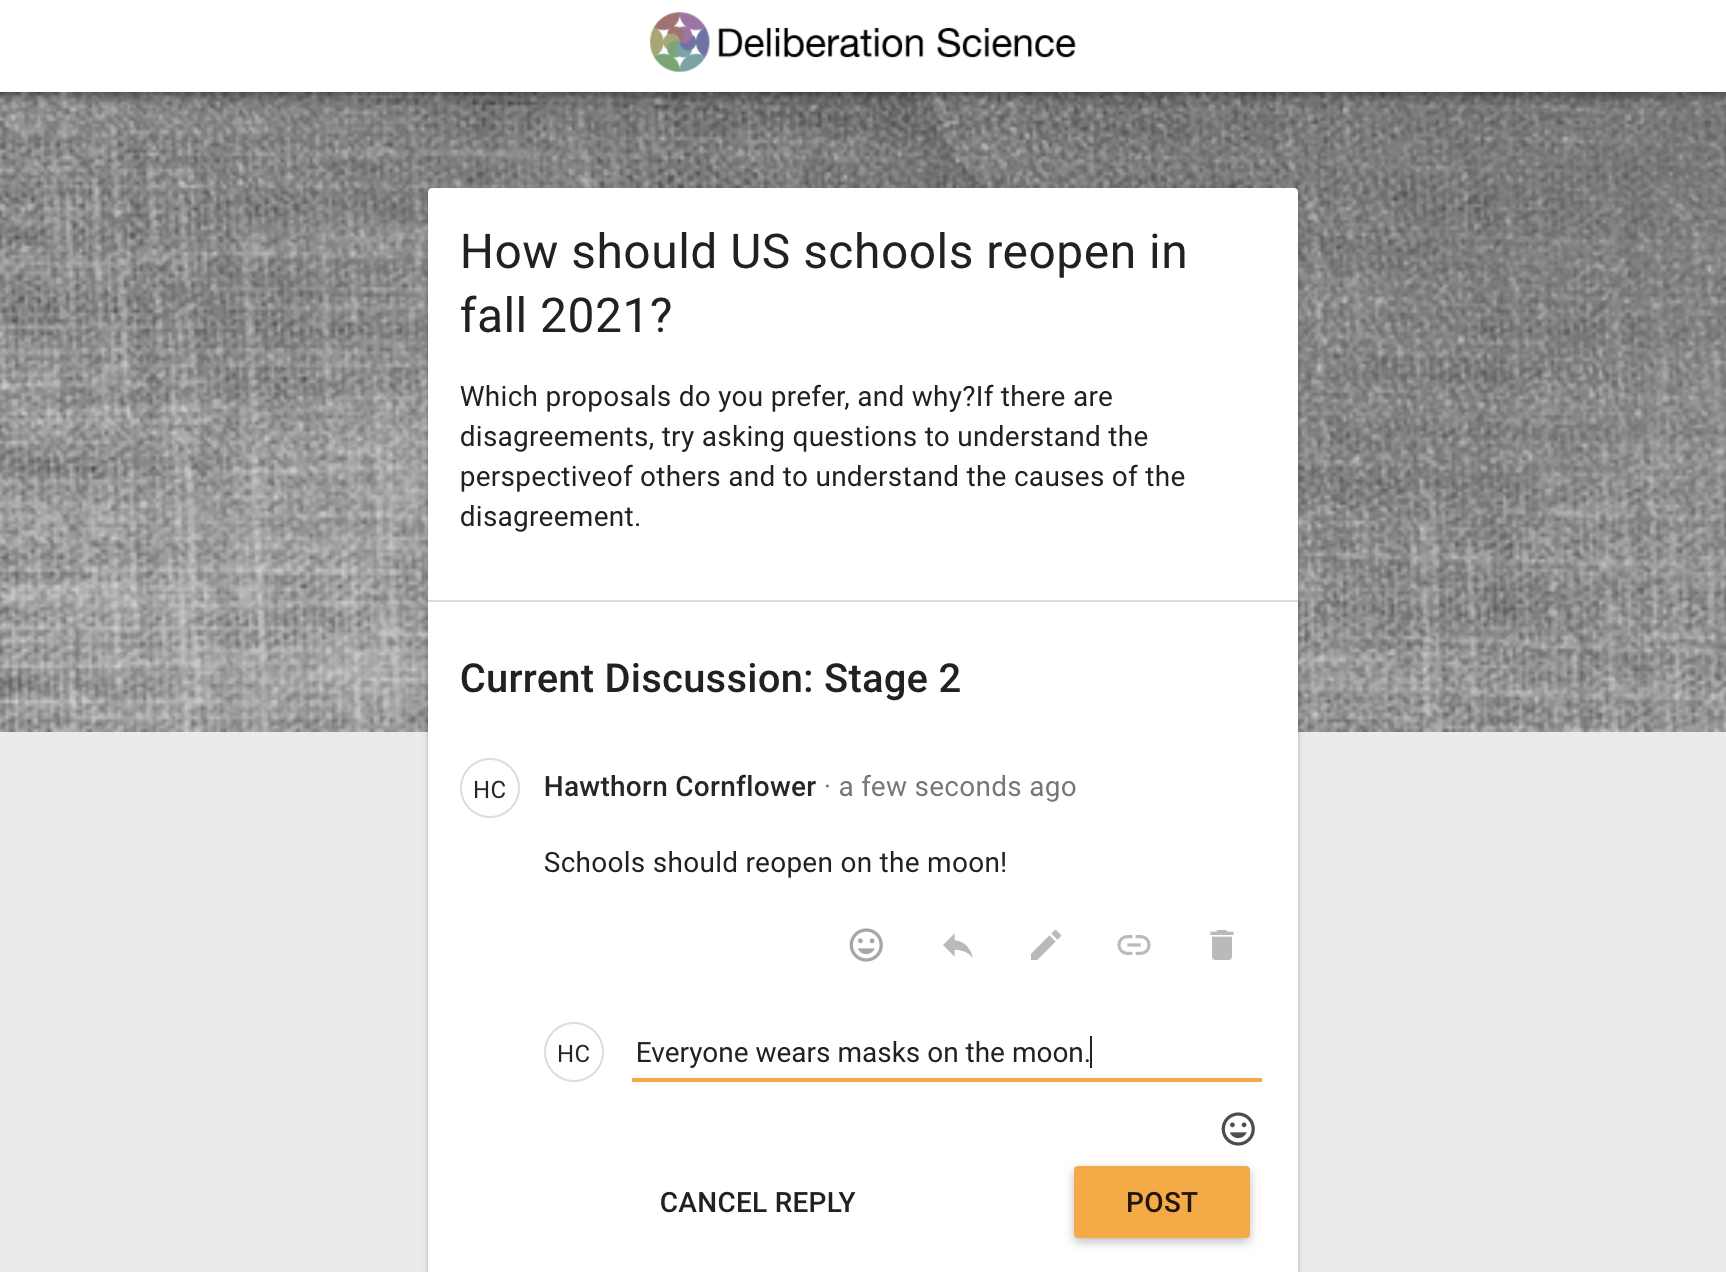
\includegraphics[width=5in]{fig/Experiment/fig-reply.png}}
\caption{Participants can perform standard forum actions, such as posting and commenting.}
\end{figure}

\begin{figure}
\label{fig:vote}
\center
\frame{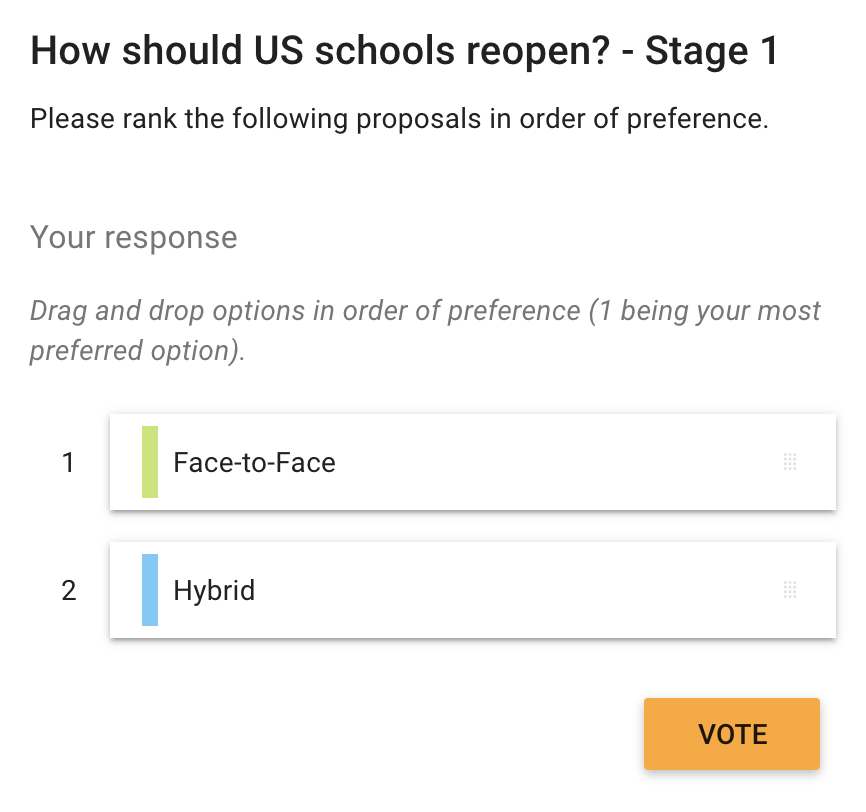
\includegraphics[width=3in]{fig/Experiment/fig-vote.png}}
\caption{Participants are presented with a ranked-choice voting screen between rounds of deliberation.}
\end{figure}

\begin{figure}
\label{fig:alias}
\center
\frame{
\includegraphics[width=3in]{fig/Experiment/fig-alias.png}}
\caption{Participants are assigned an alias for the duration of the experiment.}
\end{figure}

\section{Pilot Studies}
Several pilot studies have already been conducted:
one in a synchronous lab setting, and two using the asynchronous online
software.
In addition to providing an opportunity to test software,
these pilot studies have provided crucial information for developing a
feasible experimental design.

The initial pilot study was conducted on December 21, 2018,
before the custom online platform was developed.
In this pilot, 18 participants engaged in a synchronous 60-minute deliberation.
Participants sat at individual computer workstations, separated by dividers.
Participants discussed the following question:
``Where should the use of electric scooters be permitted?''
Participants were placed in a single treatment group, and divided into 4
pods of size 4--5.
These pods were reassigned using the random-pod method for a total of three
rounds.
The deliberation took place in chat rooms running the free and open-source
OTree online experiment software \cite{chen_otreeopen-source_2016}.

The second pilot took place after the initial development of the custom online
platform, from August 24, 2020 through August 32, 2020.
In this pilot, 7 participants engaged in an asynchronous deliberation over the
course of 7 days.
Participants were assigned to a single treatment group using network deliberation
with random-pod assignment.
Pods were size 4, and there were 3 rounds (2, 2, and 3 days).
Participants were researchers considering a week-long collaboration and
deliberated on the following question:
``What is your current preference for week of science topics?''

The third pilot took place from August 23, 2021 through August 29, 2021.
Participants deliberated on the following question:
``How should schools in the US reopen for fall 2021?''
Participants were recruited on reddit and Twitter.
18 participants were enrolled (excluding several identified as fake accounts).
These participants were divided between a conventional deliberation control
group and a random-pod treatment group.
The random-pod treatment group had two pods of size 5.
Deliberation was divided into 3 rounds (2, 2, and 3 days).

In these pilots, participants showed quantitative and qualitative evidence of
changing their preferences over the course of deliberation.
Here is an example of one such interaction:
\begin{quote}
{\bfseries Aspen Sunflower:} Even though my \#1 choice includes mandatory vaccinations, I know it's not possible due to school starting now AND MDHS can't mandate it yet. Based on previous stage, I think most seemed to want vaccinations but also wanted options. One option doesn't fit all students.

{\bfseries Aspen Poppy:} Major gap in my understanding here! The schools do not mandate vaccines for students, the state does. For the 12-17 age group, the vaccine is authorized under emergency use, full FDA approval is pending. This strengthens my desire to see hybrid learning with smaller in person groups and vaccinated staff.
\end{quote}

While the pilots did not have enough participants to identify any differences
in the evolution of preferences between different treatment groups,
evidence that preferences do change through deliberation affirms the central
assumption of this dissertation and further motivates the question of how
communication network structure influences that evolution.

\section{Experimental Design}

This section describes the experimental design of the proposed field experiment.
In this experiment, participants will use a pseudonymous online platform
to deliberate on a policy issue.
The deliberation will take place asynchronously, over a period of several days.
At several times throughout the deliberation,
participants will complete a ranked-choice poll regarding the policy issue,
allowing the evolution of their preferences to be tracked over the course of the
experiment.
Depending on opportunity and necessity, multiple waves of deliberation may
be conducted, each with a distinct policy issue and set of participants.


\subsection{Deliberative Topic}
The policy issue chosen as the topic of deliberation is a crucial component
of the experiment.
The topic will be chosen carefully according to several criteria.
The chosen policy issue must be:
\begin{itemize}
\item Relevant to the experimental population;
\item Amenable to participants changing their preferences based on new information or reasoning;
\item Amenable to a predefined list of proposed solutions;
\item Sufficiently complex to have three or more proposed solutions;
\item Timely, but unlikely to be influenced by current events during the deliberation.
\end{itemize}
Examples of policy issues meeting these criteria include:
\begin{itemize}
\item ``Where should the use of electric scooters be permitted?''
\item ``Given the COVID-19 pandemic, how should schools in the US reopen in Fall 2021?''
\end{itemize}


\subsection{Participant Recruitment and Incentives}
Participants will be recruited using several methods.
Participants will be recruited individually through posts on web forums
relevant to the policy question (e.g., reddit, facebook groups)
and to relevant email lists.
Participant pools will also be utilized,
including lists of previous participants
who have expressed interest in future studies
and the UMSI Online Recruitment System for Economic Experiments.
Individual participants will also be recruited using promoted posts and
advertisements on Twitter, Facebook, etc.
Separately, participants may also be recruited through partnership with
community groups who wish to try network deliberation as part of an organizational
decision-making strategy.
The number of such collaborations will depend on the number of interested
partner organizations that have decisions amenable to network deliberation
over the course of the experiment.

In order to incentivize participation and to compensate participants fairly
for their time,
participants who complete the deliberation and pre/post-experiment surveys
will be compensated financially.
Participants will be paid a predetermined fixed amount in order to
minimize the effect of the compensation on their deliberative behavior and
expressed preferences.


\subsection{Experimental Protocol}

Before the deliberation period begins,
participants will complete a short demographic survey.
This survey will enable the identification of sample bias in age, gender, race,
and other demographic factors.

Participants will be randomly assigned to one of three treatment/control groups
at time of enrollment:
\begin{description}
\item[Control]{
The control group will engage in conventional single large group deliberation.
Posts and comments made by participants in the control group will be visible
to all others in the control group for the entire duration of the deliberation.}
\item[Network Deliberation (Efficient)]{
Participants in this treatment group will be divided into small
(4--5 participant) pods.
Posts and comments made by participants in this treatment group will only be
visible to others in their current pod.
All participants will be assigned to a new pod at the beginning of each round
of deliberation using the random-pod assignment method,
producing a structurally efficient communication network.}
\item[Network Deliberation (Inefficient)]{
Participants in this treatment group will be divided into small
(4--5 participant) pods.
Posts and comments made by participants in this treatment group will only be
visible to others in their current pod.
All participants will be assigned to a new pod at the beginning of each round
of deliberation using the long-path assignment method,
producing a structurally inefficient communication network.}
\end{description}

The deliberation period will be divided into a predetermined number of {\em rounds},
each lasting a fixed length of time.
Present plans are to divide the deliberation period into three stages of two days
each.
However, these numbers may be adjusted to ensure time timeline of the
deliberation is consistent with any constraints imposed by specific policy issues.
Before and after each stage, participants will be asked to rank the proposed
solutions to the policy question according to their individual preference.
During each round, participants will be shown a discussion prompt and will be
able to post a response to that prompt.
Example prompts are shown in Table \ref{tab:prompts}.
Participants will be able to view and comment on the posts of other participants
assigned to the same pod.
Participants will also be able to view posts and comments that were visible to them
in previous rounds, but will no longer be able to interact with or reply to
those posts and comments.

\begin{table}
\center
\label{tab:prompts}
\begin{tabular}{|p{0.3in}|p{3.6in}|}
\hline
Stage & Prompt \\
\hline
1 &
Which proposals do you prefer, and why?
If there are disagreements, try asking questions to understand the perspective
of others and to understand the causes of the disagreement.
\\
\hline
2 & In the previous round of discussion, what opinions and reasoning did you
observe in your group?
How much agreement was there?
Were there any disagreements or conflicts?
If so, what were the sources of conflict, and how might they be resolved?
\\
\hline
3 &
What seem to be the most popular opinions?
Do you agree with them?
Has your opinion changed over the course of the discussion?
\\
\hline
\end{tabular}
\caption{Example prompts for each round of deliberation.}
\end{table}

\section{Quantitative Analysis}

The primary quantitative data will be the results of the ranked-choice
polls conducted before and after each stage of deliberation.
These results represent individual participants' stated preferences at multiple
time points.
Standard tools from social choice theory can be applied to such rank-ordered
preferences \cite{arrow_social_2012, brandt_computational_2012}.
At each time, these preferences can be aggregated into a {\em preference profile}
representing the collective preferences of all participants in a treatment group.
Preference profiles can be used to aggregate individual preferences into a single
ranking via a {\em social welfare function}.
Similarly, preference profiles can be used to select a single winner via a
{\em social choice function}.
These social choice and social welfare functions represent voting methods.
Different voting methods can potentially yield different results for the same
preference profile.
However, the more similar preferences are across individual participants,
the more likely it is that different voting methods will yield the same winner
or social ranking.
For example, when one proposal beats all others in pairwise contests, it is known as the
{\em Condorcet winner}.
Many voting methods yield the Condorcet winner when it exists, but the existence
of a Condorcet winner is not guaranteed.

For the purposes of this dissertation, the preference profiles will be used
to quantify agreement and conflict over the course of deliberation.
Within social choice theory, agreement can be defined by a {\em consensus class},
a set of preference profiles meeting one of several consensus criteria
\cite{elkind_rationalizations_2016}.
Examples include strong unanimity (of rank orders),
unanimity (of winners),
majority (existence of majority),
Condorcet (existence of Condorcet winner),
and transitivity (of social preference).
On the most restrictive end, in strong unanimity and unanimity,
all decision-makers prefer the same alternative.
In contrast, transitivity only requires that the social preferences induced by
individual preferences are transitive.
Distance-rationalizable voting systems are defined by projecting the preference
profile onto the nearest consensus profile according to a suitable distance.
For example, Dodgson's method \cite{dodgson_method_1876, brandt_computational_2012}
defines a distance based on swapping adjacent entries in individual preference profiles.
However, for most voting systems,
finding the consensus profile that minimizes distance is NP-Hard
\cite{elkind_rationalizations_2016}.
Social choice theory also provides measures of distances between two individual
preference rankings.
These measures can be extended to create measures of agreement for entire
preference profiles that can be calculated efficiently.

One possibility is to measure the distance from strong unanimity.
Two such methods will be used to analyze the results of the deliberation experiment:
the mean Kendal tau metric and the mean Spearman correlation.
The Kendal tau metric is the number fraction of pairwise contests that have
different results between two profiles \cite{kendall_new_1938}.
By averaging this measure over all pairs of members, an overall measure of agreement can be calculated for the group.
This measure does not incorporate information about win/loss margins,
only whether an alternative wins or loses.
To quantify the win/loss margin, the mean Spearman correlation will be used.
The Spearman correlation is the linear coefficient of correlation between the
rank orders of alternatives for two voters \cite{spearman_proof_1904}.
As with Kendall tau, the Spearman correlation can be averaged over all pairs of
members to determine a measure of agreement for the entire group.
It must be noted that representing agreement with a single number will inevitably
ignore important information.
Neither of these measures distinguishes a small number of voters disagreeing
on many comparisons from a large number of voters disagreeing on a few.
The Spearman correlation is also unable to distinguish these from situations in
which a small number of voters disagree by a very large margin.

While unanimity might be preferred,
it may sometimes be more realistic to focus on transitivity.
This consensus class requires only that the social preferences between pairs
of alternatives are transitive.
Such preference profiles guarantee that a Condorcet winner will exist,
bringing many different voting methods into agreement on which should win.

The deviation from transitivity will be qunatified by counting the number
of ranked-pair violations.
When performing a vote by the Tideman ranked pair system,
the relative order of two alternatives in the social preference is
determined by the winner of a pairwise vote,
except in the special case that contests with a higher margin have already
constrained their order due to transitivity.
In the latter case, the winner of the pairwise contest may have a lower
position in the social preference.
If this situation occurs, the social preference is intransitive and there may
not be a Condorcet winner.
Each such pair represents a contest violating the social ranking,
so the fraction of such pairs
can be used to quantify the strength of intransitivity in the group’s preferences.
This measure has the property that a Condorcet winner is guaranteed when the value is 0.



\section{Power Analysis}
The minimum number of participants required is determined by a number of factors.
First, the long-path pod assignment method results in a minimum number of pods,
determined by the chosen parameters.
Specifically, the pod assignments for each round beyond the first are determined
by a unique prime number,
and the number of pods is a multiple of that prime.
For $T=3$ rounds, two primes are necessary and choosing the lowest two (2, 3)
yields the lowest minimum number of pods: 3.
For all pods to have at least 4 members, the minimum number of participants in
the long-path treatment is 12.

The two network deliberation treatments must also have meaningfully different
structural properties,
which also necessitates a minimum number of participants.
Structural differences between these two networks become more pronounced
with a greater number of participants.
While properties such as the broadcast time (see Chapter \ref{chap:abm})
and average geodesic length can be used to compare the structural efficiency of
two networks,
they encounter a problem for these particular networks
when there is a small number of rounds:
for many pairs of individuals, no path will exist.
In practical terms,
an idea proposed by one participant may not have a plausible
path to reach some of the other participants by the end of the deliberation,
even if that idea is repeatedly shared by all who encounter it.
As an alternative, a form of k-connectivty can be used to measure
structural efficiency.
The k-connectivity is simply the fraction of possible paths that exist.
In other words, if each participant broadcasts a message, and that message is
repeated by all who encounter it, what is the average fraction of participants
a broadcast will reach?
Figure \ref{fig:kcon} shows the k-connectivity as a function of number of
participants for both the long-path and random-pod deliberation networks.
While there is no clear threshold for the necessary number of participants,
choosing a k-connectivity of $0.5$ (half of possible paths exist) seems a
reasonable heuristic.
For the chosen parameters, 35 or more participants are necessary to produce
a random-pod network with $>0.5$ k-connectivity and
a long-path network with $<0.5$ k-connectivity.

Combining the above considerations,
an absolute minimum of 12 participants per treatment is necessary to conduct
a wave of the experiment,
and a minimum of about 35 participants per treatment group is necessary to
observe differences between the network deliberation treatment conditions.

\begin{figure}
\label{fig:kcon}
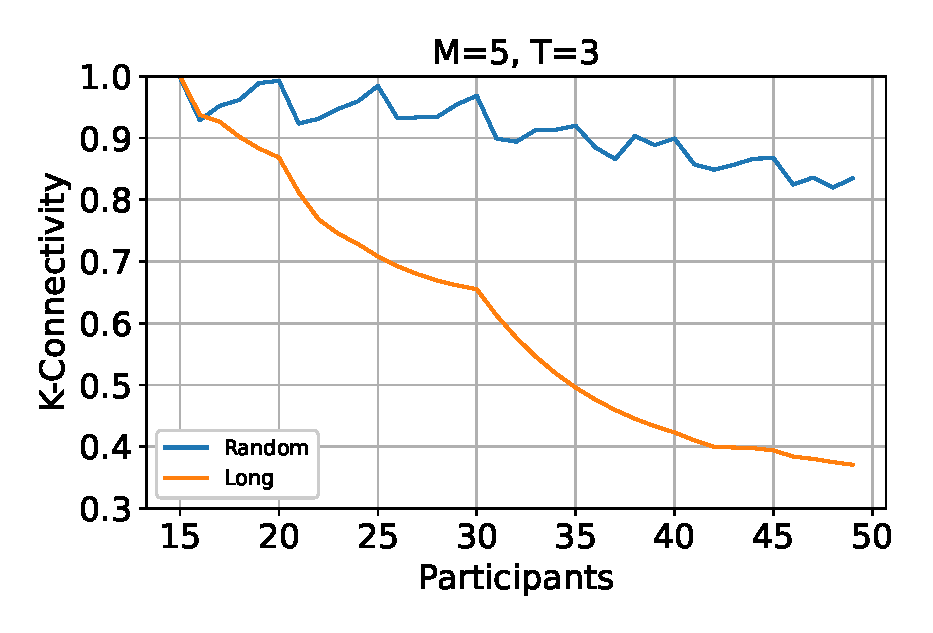
\includegraphics[width=5in]{fig/Experiment/fig-kcon.eps}
\caption{The k-connectivity of long-path and random-pod network deliberation
networks for $T=3$ stages and a pod size of $M=5$.}
\end{figure}

\section{Qualitative Analysis}
In addition to quantitative data,
qualitative data will also be collected in conjunction with
the deliberation experiment.
These data will be used to corroborate the results of quantitative
analysis and to achieve a richer understanding of individual participants'
experience of network deliberation,
as well as to as well as identify common themes that may provide
insight into the strengths and weaknesses of network deliberation.

The text of participants' posts and comments throughout the deliberation
will be kept for analysis.
This text can potentially be used to identify deliberative behaviors that
lead to changes in preferences.
Similarly, this text can be used to track the diffusion of specific keywords,
arguments, and influence through the communication network.

A subset of participants will be randomly selected to participate in
60-minute semi-structured interviews about their experience.
The interview script can be found in Appendix \ref{apx:interview}.
These interviewed will be transcribed and qualitatively coded using a
grounded theory approach.
The initial code book will be developed by open-coding pilot study transcripts
and an initial subset of interview transcripts.


